\documentclass[a4paper,12pt]{article}
\usepackage[hmargin=2cm,top=4cm,headheight=65pt,footskip=45pt]{geometry}
\usepackage[utf8]{inputenc}
\usepackage{graphicx}
\usepackage[hidelinks]{hyperref}
\usepackage{array}
\usepackage{lastpage}
\usepackage{lipsum}
\usepackage{fancyvrb}
\usepackage{color}
\usepackage{fancyhdr}
\usepackage{amsmath}
\usepackage{enumitem}
\usepackage{titlesec}
\usepackage{floatrow}
\newfloatcommand{capbtabbox}{table}[][\FBwidth]

\definecolor{customGray}{RGB}{128,128,128}
%\definecolor{Eblue}{RGB}{0,21,87}
%\definecolor{Eblue}{rgb}{0.2, 0.2, 0.6}
\definecolor{Eblue}{rgb}{0.0, 0.18, 0.39}
%==============Header & Footnote==============

\pagestyle{fancy}
\renewcommand{\headrulewidth}{0pt}
\fancyhead[C,CO,L,LO,R,RO]{}
\fancyhead[C]{%
          \begin{tabular}{|m{3.0cm}|m{10.0cm}|m{2.5cm}|}
          \hline
          \centering\vspace{1.75mm}
\includegraphics[scale=0.275]{logo.pdf} &
          \centering
          {\footnotesize {\sf UNIVERSIDAD EAFIT\\ SCHOOL OF ENGINEERING\\
          \vspace{-1mm}DEPARTMENT OF SYSTEMS AND INFORMATICS}} &
          \centering
          \footnotesize{Page \thepage\ de \pageref{LastPage}\\
          ST245\\
          \vspace{-0.75mm}Data Structures
          }\tabularnewline
          \hline
          \end{tabular}%
}
\fancyfoot[C,CO,L,LO,R,RO]{}
\fancyfoot[C]{
          \begin{centering}
            \textcolor{customGray}{{\footnotesize {\sf Professor Mauricio Toro Bermúdez\\
            Phone: $(+57) (4) 261 95 00$ Ext. $9473$. Office: $19 - 627$\\
            \vspace{-1mm}E-mail: mtorobe@eafit.edu.co}}}
        \end{centering}
}

%=============CustomEnumItem===========

\setlist[enumerate]{label=\color{Eblue}\textbf{\roman*.}}

%=============CustomSecSubSec==========

\titleformat{\section}[hang]
{\normalsize\bfseries\itshape\color{black}}{\bfseries\itshape\color{Eblue}\thesection)}{2.5mm}{}

\titleformat{\subsection}[hang]
{\normalsize\bfseries\itshape\color{black}}{\bfseries\color{Eblue}\thesection.\alph{subsection}.}{2.5mm}{}

%==============Title==============

\title{\color{Eblue}\textbf{Laboratory practice No. 2: Big O Notation}}
\author{
  \textbf{Juan S. Cárdenas Rodríguez}\\
  Universidad EAFIT\\
  Medellín, Colombia\\
  jscardenar@eafit.edu.co
\and
  \textbf{David Plazas Escudero}\\
  Universidad EAFIT\\
  Medellín, Colombia\\
  dplazas@eafit.edu.co
}

%=============Document=============
\begin{document}
  \maketitle
  \thispagestyle{fancy}

  \section{ONLINE EXERCISES (CODINGBAT)}
  \subsection{Recursion I}
    \begin{enumerate}
      \item \begin{Verbatim}
      public int countPairs(String str) {             // c0
        if (str.length() <= 2) {                      // c1
          return 0;                                   // c2
        } else if (str.charAt(0) == str.charAt(2)) {  // c3
          return 1 + countPairs(str.substring(1));    // c4 + T(n-1)
        } else {                                      // c4
          return countPairs(str.substring(1));        // T(n-1)
        }
      }
      \end{Verbatim}
      Complexity of \texttt{countPairs} can be writen as:
      \begin{equation*}
        T\left( n \right)=\left\{\begin{array}{cc} c_{0}+c_{1}+c_{2} & n\leq 2 \\ c_{3}+c_{4}+T\left( n-1 \right) & n>2\end{array}\right.
      \end{equation*}
      Solving the recursive equation yields:
      \begin{equation*}
        T\left( n \right)=(c_3+c_4)n+k
      \end{equation*}
      Therefore, $T(n)$ is $O(cn+k)$ and applying the sum and product rule $T(n)$ is $O(n)$.


    \section{SIMULATION OF PROJECT PRESENTATION QUESTIONS}
    \subsection{ArrayMax}
    \begin{figure}[ht]
      \begin{floatrow}
        \ffigbox{
          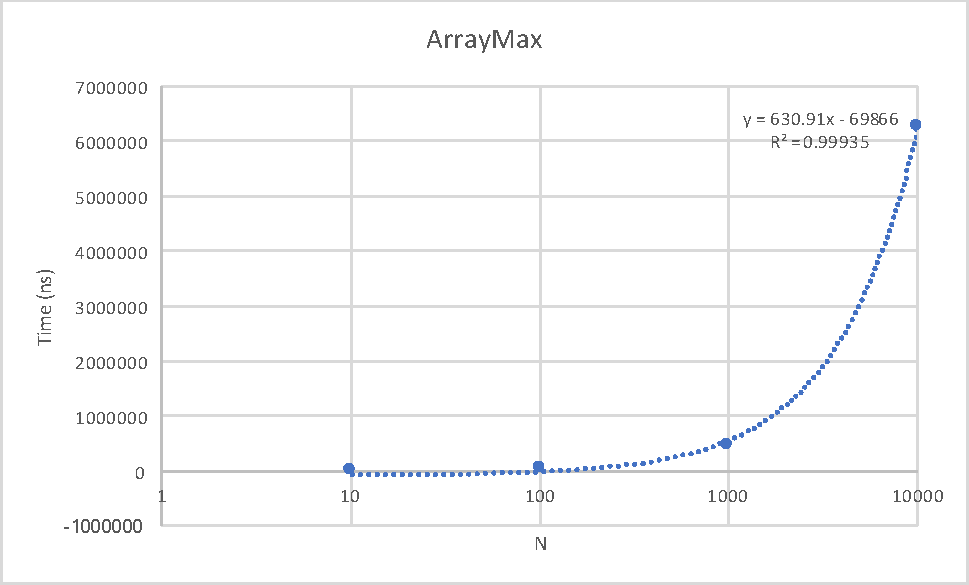
\includegraphics[scale=0.45]{ArrayMax.pdf}
        }{
          \caption{Time vs. N for ArrayMax}
        }
        \capbtabbox{
          \begin{tabular}{cc}
            \hline
            \textbf{N} & \textbf{Time (ns)} \\ \hline
            10         & 6000               \\
            100        & 27000              \\
            1000       & 346000             \\
            10000      & 6717000            \\ \hline
          \end{tabular}
        }{
          \caption{ArrayMax's data.}
        }
      \end{floatrow}
    \end{figure}

    \section{EXAM SIMULATION}
    \begin{enumerate}
      \item $\texttt{start}+1,\quad \texttt{nums},\quad \texttt{target}$
      \item a) $T(n) = T(n/2) + C$
      \item $n-a, a, b, c$\\
      res, solucionar($n-b,a,b,c$)+1\\
      res, solucionar($n-c,a,b,c$)+1
      \item e) La suma de los elementos de a y es $O(n)$.
    \end{enumerate}


    \newpage
    \bibliographystyle{plain}
    \bibliography{Lab.bib}
\end{document}
